\documentclass[12pt, a4paper]{report}
\usepackage[utf8]{inputenc}
\usepackage[russian]{babel}

\usepackage[T2A]{fontenc}
%for additional symbols
\usepackage{textcomp}
\usepackage{amsmath}
\usepackage{amssymb}
\newcommand{\R}{\mathbb{R}}

% for indent first paragraph within section
\usepackage{indentfirst}

%for text boundaries
\usepackage[a4paper, left=15mm, right=15mm, top=15mm, bottom=15mm]{geometry}

%for some mathematical things
\usepackage{amsmath}

%for pictures
\usepackage{graphicx}
\usepackage{alltt}

\usepackage{listings}
\usepackage{color}
\usepackage{xcolor}
\usepackage{hyperref}


\definecolor{mygray}{rgb}{0.4,0.4,0.4}
\definecolor{mygreen}{rgb}{0.0,0.16,0.67}
\definecolor{myorange}{rgb}{1.0,0.25,0}
\definecolor{myblue}{rgb}{0.17,0.27,0.53}

\lstset{
basicstyle=\footnotesize\sffamily\color{black},
commentstyle=\color{mygray},
frame=single,
numbers=left,
numbersep=5pt,
numberstyle=\tiny\color{myblue},
keywordstyle=\color{mygreen},
showspaces=false,
showstringspaces=false,
stringstyle=\color{myorange},
tabsize=3,
extendedchars=\true,
inputencoding=utf8,
breaklines=true
}



\graphicspath{{./Screenshots/}}


\begin{document}
	\begin{titlepage}
  \begin{center}
    \vspace{2cm}
    Санкт-Петербургский Национальный Исследовательский Университет\\
    Информационных Технологий, Механики и Оптики

    \vspace{6cm}

    Кафедра Систем Управления и Информатики

    \vspace{3cm}
    \textbf{Экзаменационная работа:\\ Написание прикладной программы на языке Python}
  \end{center}
  \vspace{4cm}
  \hfill
  \parbox[top][3cm][t]{3cm}{Выполнил:}
  \parbox[top][3cm][t]{3cm}{
  Антипов В.А.}
  \\

  \hfill
  \parbox[right][3cm][t]{3cm}{Проверили:}
  \parbox[right][3cm][t]{3cm}{
  Мусаев А.А.}

  \vfill
  \begin{center}
  Санкт-Петербург \\ 2018
  \end{center}
\end{titlepage}
	\newpage
\section*{\centeringЗадача}
Необходимо написать программу для нахождения функциональной зависимости параметров. В качестве параметров дана таблица экспериментальных измерений в GoogleSheets. Зависимость параметров ищется по трем заданным функциям:
$$ y = A \cdot exp(t), \quad y = A \cdot t^2, \quad y = A \cdot t + B $$
Также программа должна учитывать введенное пользователем максимальное относительное отклонение связи. Отклонение задается пользователем в процентах. Результат выполнения программы должен сохраняться в текстовый файл в виде:\\
"Параметр 1 связан с Параметром 2, зависимость линейная".
	\newpage
	\section*{\centering Выполнение}
	
	\subsection*{Настройка аккаунта и установка пакетов}
	Для обращения к Google таблицам необходимо создать учетную запись и получить доступ к GoogleSheets API и GoogleDrive API.\\
	
	\paragraph{Для этого необходимо:\\
	}
	- Создать Google Аккаунт, если он отсутствует.\\
	- Войти в \textit{Google API Console}\\
	- Cоздать новый проект и подключить к нему GoogleSheets API и GoogleDrive API.\\
	- Сконфигурировать JSON ключ данной учетной записи для подключения к GoogleSheets через OAuth 2.\\
	- Добавить аккаунт "робота" в группу разработчиков проекта (таблицы).\\
    \begin{center}
        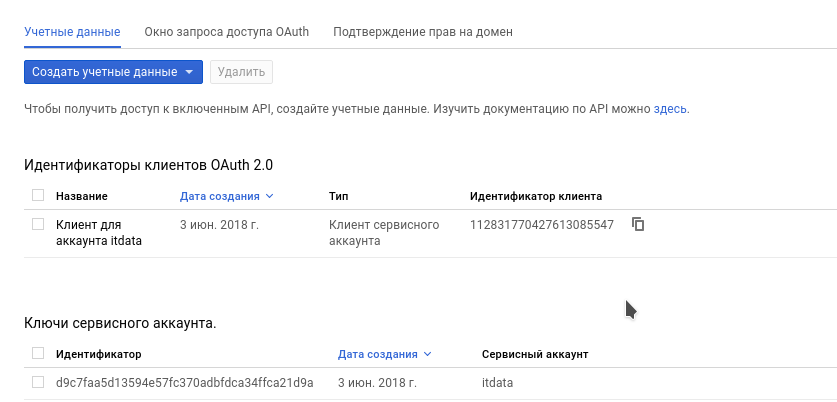
\includegraphics[width=0.7\textwidth]{OAuth2.png}
        \textit{Созданные сервисный аккаунт и полученный json ключ}
    \end{center}
	
	Теперь перейдем к установке пакетов Python. Воспользуемся удобным пакетным менеджером Pip3 для установки пакетов gspread и OAuth2Client, необходимых для работы с google таблицами и аутентификации  в сервисах google.
	\begin{lstlisting}
    pip3 install gspread oauth2client
    \end{lstlisting}
    
    \subsection*{Написание программы}
    Программа разделена на несколько частей, сформировавших пакеты:\\
    1) Аутентификация в GoogleSheets и парсинг данных из таблицы.(\textit{GoogleTableHandler}\\
    2) Установка и поиск функциональной зависимости.(\textit{DependenceSolver})\\
    3) Вывод результатов и прогресса решения в консоль.(\textit{Output})\\
    
    \paragraph{1) Аутентификация в GoogleSheets и парсинг данных из таблицы.(\textit{GoogleTableHandler})\\
    }
    
    Модуль AuthManager предназначен для аутентификации в сервисах google посредством протокола OAuth2. OAuth2 - это сравнительно новый протокол для авторизации, основанный на http-запросах. С помощью него можно выдавать права другим программам, таким как наша, на редактирование данных от лица пользователя без аутентификации под новым пользователем.\\
    
    Модуль \textit{AuthManager}:
    \begin{lstlisting}[language=Python]
    def authorized():
        while True:
            autkey = input("Введите путь до ключа аутентификации: ")
            scope = ['https://spreadsheets.google.com/feeds', 'https://www.googleapis.com/auth/drive']
            try:
                creds = ServiceAccountCredentials.from_json_keyfile_name(autkey, scope)
                client = gspread.authorize(creds)
                print("[Google Sheets] Authentification Complete!")
                return client
            except FileNotFoundError:
                print("Файл "+ autkey + " не найден!")
            except json.decoder.JSONDecodeError:
                print("Файл не является ключом!")
                continue
    \end{lstlisting}
    
    Для подключения используется json-ключ, хранящий в себе данные(ключ) для доступа к возможностям аккаунта без аутентификации (логина и пароля).\\
    После запроса ввести путь до json-ключа в программе записываются в лист сервисы для которых мы хотим получить \textit{authorization code} (код полученный для приложения от сервера, необходимый для последующего формирования запросов).
    Далее происходит формирование полномочий и авторизация:
    
    \begin{lstlisting}[language=Python]
    ServiceAccountCredentials.from_json_keyfile_name(autkey, scope)
    client = gspread.authorize(creds)
    \end{lstlisting}
    
    Если будет поймана ошибка о неверности json ключа или его отсутствии - пользователь будет вынужден ввести путь до него еще раз.\\
    После успешной авторизации метод \textit{def authorized()} вернен обьект типа \textit{client}, с помощью него и будет происходить получение и запись данных в таблицу.\\
    
    Обработкой данных из таблицы занимается класс \textit{TableManager}. Класс формирует удобные для обработки листы с параметрами из полученной с помощью \textit{client}-a таблицы.\\
    Метод класса \textit{def \_\_openTable(self)} открывает таблицу по имени или url с помощью \textit{client}-a и в случае возникновения ошибки - говорит об этом.
     \begin{lstlisting}[language=Python]
    def __openTable(self):
        try:
            if re.match("http", self.__tablename) :
                table=self.__client.open_by_url(self.__tablename).sheet1
            else:
                table = self.__client.open(self.__tablename).sheet1
        except gspread.exceptions.SpreadsheetNotFound:
            print("[ERROR]: You can not open this GoogleSheets!")
            exit(5)
        return table
    \end{lstlisting}
    
    Метод класса \textit{def getParamList(self)} формирует список параметров в листе проверяя корректность полей, отсутствие данных в ячейке и переводя все числа в тип \textit{float128} для работы с длинной арифметикой с помощью NumPy.
    \begin{lstlisting}[language=Python]
    def getParamList(self):
        tableList= self.__getTableListfromEdit()
        paramList = []
        countMetrics = 0
        for parameter in tableList:
            if re.match("Parameter", parameter[0]):
                if (countMetrics != 0) and (len(parameter[1:]) != countMetrics):
                    print("Count parameter error!")
                    exit(6)
                paramList.append(list(map(float128, parameter[1:])))
                countMetrics = len(paramList[0])
        return paramList
    \end{lstlisting}
    
    \newpage
    Таблица принимается в следующем виде:
    \begin{center}
        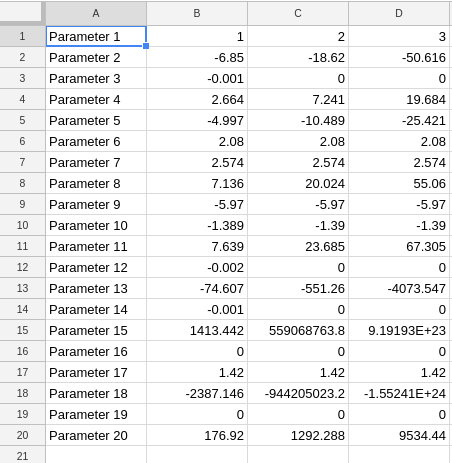
\includegraphics[width=0.7\textwidth]{TableForm.png}\\
        \textit{Тестовая сгенерированная таблица параметров.}
    \end{center}
    
    Метод \textit{def setParamList(self, list)} позволяет записывать построчно в таблицу данные полученные в качестве листа, как параметра вызова. Данный метод будет необходим для записи в таблицу тестовых случайно сгенерированных данных для проверки работы программы.
    \begin{lstlisting}[language=Python]
    def setParamList(self, list):
        self.__table.clear()
        for i in range(len(list)):
            self.__table.delete_row(i+1)
            self.__table.insert_row((["Parameter " + str(i+1)] + list[i]), i+1)
    \end{lstlisting}
    
	
	
	\paragraph{2) Установка и поиск функциональной зависимости.(\textit{DependenceSolver})
    \\
    }
	
	Основой данного пакета и всей программы в целом является класс \textit{DependenceFinder}. В данном классе реализованы методы для поиска функциональной зависимости параметров.\\
	Алгоритм поиска зависимостей основан на МНК - методе наименьших квадратов. Метод наименьших квадратов наиболее прост в программной реализации. Также был вариант использовать метод дифференцирования, но он был отсечен, ввиду малого количества экспериментальных точек, что критично для численного дифференцирования. Сам метод заключается в поиске неопределенных коэффициентов уравнения, так чтобы сумма квадратичных ошибок отклонения экспериментальных данных от этого уравнения была минимальной, т.е:\\
	$$e = y-y^* \quad S=\sum_{i=1}^{n} e^2 $$
	, где: $e$ - отклонение, $y$ - вид функции по которой будет происходить аппроксимация, $S$ - сумма квадратов ошибок. Принцип МНК именно в нахождении таких коэффициентов у функции $y$, чтобы $S \to 0$.
	
	Выведенные формулы для аппроксимации данных нам функций:\\

	1) Линейная аппроксимация ($y=A\cdot x + B$):
	$$A = \dfrac{ n\cdot \sum_{i=1}^n (y^*_i \cdot x_i) - \sum_{i=1}^n y^*_i \cdot \sum_{i=1}^n x_i} {n\cdot \sum_{i=1}^n x_i^2 + (\sum_{n=1}^n x_i)^2} \quad B = \frac{\sum_{i=1}^n y^*_i - A \cdot \sum_{i=1}^n x_i}{n}$$
	
	2) Экспоненциальная аппроксимация ($y = A \cdot e^x$):
    $$ A = exp \Bigr( \frac{\sum_{i=1}^n(ln (y^*_i) + x_i)}{n}\ \Bigl)$$

    3) Квадратичная аппроксимация ($y = A \cdot x^2$)
    $$ A = \frac{\sum^n_{i=1} x_i^2 \cdot y_i}{\sum^n_{i=1} x_i^4}$$

    \begin{lstlisting}[language=Python]
    def expAproxMNK(self, param1, param2):
        if not self.__checkAriphmetics(1e-10, 1e+20, 1e-10, 1e+5, param1, param2, True):
            return [[0.0], 0.0, False]
        return self.__getAexp(param1, param2)

    def linearAproxMNK(self, param1, param2):
        if not self.__checkAriphmetics(1e-10, 1e+20, 1e-10, 1e+20, param1, param2, False):
            return [[0.0, 0.0], 0.0, False]
        return self.__getABlin(param1, param2)


    def quadAproxMNK(self, param1, param2):
        if not self.__checkAriphmetics(1e-10, 1e+20, 1e-10, 1e+10, param1, param2, False):
            return [[0.0], 0.0, False]
        return self.__getAquad(param1, param2)
    \end{lstlisting}

    После поиска коэффициентов, происходит подсчет максимального отклонения экспериментальных данных от значения аппроксимирующей функции и сравнение этого отклонения с введенным пользователем максимальным отклонением.\\

    Метод класса \textit{def \_\_checkAriphmetics(self, minparam1, maxparam1, minparam2, maxparam2, param1, param2, checkNegativeNumber)} проверяет принадлежат ли параметры интервалу допустимых числовых значений, это было введенно для отсечения вычислений приводящих к переполнению памяти, выделенной на переменную. Также подобная проверка отсекает поиск функциональной зависимости при неизменных параметрах. В случае обнаружения недопустимо малых, повторяющихся или недопустимо больших чисел метод возращает False, иначе True. 

    \begin{lstlisting}[language=Python]
    def __checkAriphmetics(self, minparam1, maxparam1, minparam2, maxparam2, param1, param2, checkNegativeNumber):
        n = len(param1)
        countzero1 = 0
        countzero2 = 0
        repeat = param2[0]
        countrepeat = 0

        for i in range(n):
            if i != 0 and param2[i] == repeat:
                countrepeat += 1
            repeat = param2[i]
            if abs(param1[i]) < minparam1 or abs(param2[i]) > maxparam1 or (checkNegativeNumber and param1[i] < 0.0):
                countzero1 += 1
            if abs(param2[i]) < minparam2 or abs(param2[i]) > maxparam2:
                countzero2 += 1
        if countzero1 != 0 or countzero2 != 0 or countrepeat != 0:
            return False
        else: return  True
    \end{lstlisting}

    В следующих методах происходит сама аппроксимация, при этом на выходе мы получаем лист, который хранит в себе результат аппроксимации, то есть: коэффициенты, максимальное найденное отклонение и флаг о прохождении проверки. Для аппроксимации было решено использовать lambda выражения для сокращения записи и удобочитаемости.\\
    
    Квадратичная аппроксимация($y=A\cdot x^2$):
    \begin{lstlisting}[language=Python]
    def __getAquad(self, param1, param2):
        maxRelError = -1
        n = len(param1)
        a = np.sum(list(map(lambda x, y: x * x * y, param2, param1))) / np.sum(list(map(lambda x: x ** 4, param2)))

        if abs(a) < 1e-10: return [[0], 0.0, False]
        for i in range(n):
            relError = -1
            if param2[i] != 0:
                relError = np.abs((a * param2[i] ** 2 - param1[i]) / (a * param2[i] ** 2))

            if relError > maxRelError:
                maxRelError = relError
        if maxRelError == -1 or maxRelError > self.__maxRelativeError:
            return [[0], 0.0, False]
        else:
            return [[a], maxRelError, True]
    \end{lstlisting}

    Линейная аппроксимация($ y=A\cdot x + B$):
    \begin{lstlisting}[language=Python]
    def __getABlin(self, param1, param2):
        maxRelError = -1
        n=len(param1)

        a = (n * (np.sum(list(map(lambda x, y: x * y, param2, param1)))) - np.sum(param1) * np.sum(param2)) / (
                    n * np.sum(list(map(lambda x: x * x, param2))) - np.sum(param2) ** 2)
        b = (np.sum(param1) - a * np.sum(param2)) / n

        if a == 0.0: return [[a], 0.0, False]
        for i in range(n):
            if param2[i] != 0.0:
                relError = np.abs(((a * param2[i] + b) - param1[i]) / (a * param2[i] + b))
            else:
                relError = np.abs(param1[i])

            if relError > maxRelError:
                maxRelError = relError

        if maxRelError == -1 or maxRelError > self.__maxRelativeError:
            return [[0, 0], 0.0, False]
        else:
            return [[a, b], maxRelError, True]
    \end{lstlisting}

    Экспоненциальная аппроксимация($y=A\cdot e^x$):
    \begin{lstlisting}[language=Python]
        def __getAexp(self, param1, param2):
        maxRelError = -1
        n = len(param1)
        a = np.exp(np.sum(list(map(lambda x, y: (np.log(y) - x), param2, param1))) / n)

        for i in range(n):
            relError = np.abs((a * np.exp(param2[i]) - param1[i]) / (a * np.exp(param2[i])))
            if relError > maxRelError:
                maxRelError = relError
        if maxRelError == -1 or maxRelError > self.__maxRelativeError:
            return [[0], 0.0, False]
        else:
            return [[a], maxRelError, True]
    \end{lstlisting}

    \paragraph{2.1) Генератор зависимостей для тестирования:
    \\
    }
    Следующий класс данного пакета \textit{TestGenerator}. В нем происходит непосредственно генерация тестовых данных для тестирования искателя зависимостей параметров. Данный класс был написан исключительно для тестирования, в нем используется random позволяюший создать случайное отклонение от желаемой функциональной зависимости. Параметры для генерации зависимости а также функция также выбираются случайно.\\

    \begin{lstlisting}[language=Python]
    def __expGen(self):
        a = random.randint(-self.__maxvalue*4, self.__maxvalue*4)/2.0
        error = random.randint(-self.__randomError, self.__randomError)/100.0
        numberparam1 = random.randint(0, len(self.__currentGenParameters)-1)
        param1 = np.array(self.__currentGenParameters[numberparam1], dtype=np.float128)
        param2 = list(map(lambda x: float(np.round(((a*np.exp(x)).real + (a*np.exp(x)*error).real), 3)), param1))
        return param2

    def __linGen(self):
        a = random.randint(-self.__maxvalue*4, self.__maxvalue * 4) / 2.0
        b = random.randint(-self.__maxvalue*4, self.__maxvalue * 4) / 2.0
        error = random.randint(-self.__randomError, self.__randomError) / 100.0
        numberparam1 = random.randint(0, len(self.__currentGenParameters) - 1)
        param1 = np.array(self.__currentGenParameters[numberparam1], dtype=np.float128)
        param2 = list(map(lambda x: float(np.round(((a * x + b) + (a * x +b) * error), 3)), param1))
        return param2


    def __quadGen(self):
        a = random.randint(-self.__maxvalue*4, self.__maxvalue * 4) / 2.0
        error = random.randint(-self.__randomError, self.__randomError) / 100.0
        numberparam1 = random.randint(0, len(self.__currentGenParameters) - 1)
        param1 = np.array(self.__currentGenParameters[numberparam1], dtype=np.float128)
        param2 = list(map(lambda x: float(np.round((a*x*x + a*x*x*error), 3)), param1))
        return param2
    \end{lstlisting}

    Класс \textit{GlobalSolver()} является оберткой для всех вышеперечисленных классов, он является основой программы, в нем создаются обьекты DependenceFinder и TestGenerator, а также определяются их параметры.\\

    В функции класса \textit{def \_\_open(self)} происходит:\\

    1) запрос ввода имени таблицы.\\
    2) обработка TableManager-ом таблицы.\\
    3) создание генератора тестовой таблицы и непосредственно сама генерация.(для конечной программы данная часть кода отсутствует).\\
    4) Получение параметров из таблицы.\\
    5) Запрос ввода имени для сохранения файла с результатами.\\
    6) Запрос ввода макимально допустимого отклонения от найденной связи.\\
    7) Создание обьекта решателя.\\

    \begin{lstlisting}[language=Python]
    def __open(self):
        self.__client = authorized()
        self.__tablename = input("Введите название гугл таблицы на вашем аккаунте или url адрес доступной таблицы: ")
        self.__tableMan = TableManager(self.__client, self.__tablename)
        #self.__gen = RandomDependGenerator(20, 1, 50)
        #self.__tableMan.setParamList(self.__gen.randomGeneratedDepend())
        self.__tableMan.getParamList()
        self.__parameters = self.__tableMan.getParamList()
        self.__outfilename = input("Введите имя файла для сохранения результатов: ")
        self.__fileWriter = OutputFileWriter(self.__outfilename)
        self.__maxRelError = float(input("Введите максимальное относительное отклонение в процентах от зависимости: "))/100.0
        self.__finder = DependenceFinder(self.__maxRelError)
    \end{lstlisting}

    В методе \textit{def solv(self)} происходит нахождение зависимостей путем перебора всех параметров, т.е. программа выполняет $n\cdot (n-1)$ итераций. Из найденных возможных связей выбирается та, что имеет наименьшее отклонение. Также здесь проинициализирован прогресс бар, для удобного мониторинга процесса расчета зависимостей.
    Обновление прогресс бара происходит каждый такт подбора связи между двумя параметрами.

    \begin{lstlisting}[language=Python]
    def solv(self):
        progressBar = ConsoleProgressBar(50, self.__countParameters*(self.__countParameters-1))
        progressBar.startProcess()
        countdep=0

        for p1 in range(len(self.__parameters)):
            for p2 in range(len(self.__parameters)):
                if p1 != p2:
                    #print(str(p1)+" "+str(p2))
                    dep = 3
                    minError = 1000000
                    resultL = self.__finder.linearAproxMNK(self.__parameters[p1], self.__parameters[p2])
                    resultE = self.__finder.expAproxMNK(self.__parameters[p1], self.__parameters[p2])
                    resultQ = self.__finder.quadAproxMNK(self.__parameters[p1], self.__parameters[p2])
                    rel=[resultL[2], resultE[2], resultQ[2]]
                    commonResultError = [resultL[1], resultE[1], resultQ[1]]


                    for i in range(len(commonResultError)):
                        if commonResultError[i] < minError and commonResultError[i] < self.__maxRelError and rel[i]:
                            minError = commonResultError[i]
                            dep = i
                    if dep != 3:
                        self.__fileWriter.writeResult(p1, p2, self.__accesDependList[dep])
                        countdep+=1
                    progressBar.updateProgress(countdep)
    \end{lstlisting}


    \paragraph{3) Вывод результатов и прогресса решения в консоль.(\textit{Output})\\
    }
     Последняя часть программы необходима для вывода результатов расчетов на экран. В этом пакете лежит класс \textit{OutputFileWriter}, необходимый для форматированного вывода результатов в файл. Его метод \textit{def writeResult} в каждой новой строке пишет то, какой параметр с каким связан и какой функциональной зависимостью.

     \begin{center}
        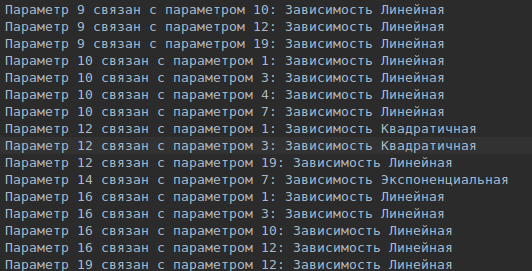
\includegraphics[width=0.7\textwidth]{output.png}\\
        \textit{Вывод результата поиска зависимостей в файл.}
    \end{center}

     \begin{lstlisting}[language=Python]
        def writeResult(self, NumberParam1, NumberParam2, type): self.__file.write("Параметр " + str(NumberParam1) + " связан с параметром " + str(NumberParam2) +": Зависимость "+ type + "\n")
     \end{lstlisting}

     Класс \textit{ConsoleProgressBar} был реализован для красивого, динамически обновляемого вывода текущего процесса расчета в консоль со шкалой заполнения. Его основой является метод \textit{def updateProgress(self, countDepend)}, в нем происходит расчет необходимого количества символов, для заполнения шкалы пропорционально рашению. Динамическое обновление данных происходит благодаря использованию потокового вывода \textit{stdout}.

     \begin{center}
        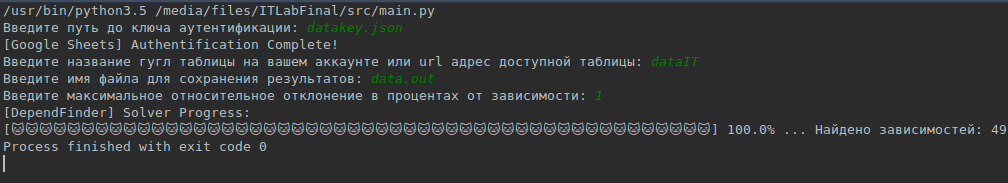
\includegraphics[width=\textwidth]{progress.png}\\
        \textit{Результат работы программы, вывод прогресса.}
    \end{center}


     \begin{lstlisting}[language=Python]
    def updateProgress(self, countDepend):
        self.__currentProgress += 1
        self.__currentSizeBar = round(1.0*self.__currentProgress * self.__sizeIterable)

        self.__bar = u'#' * self.__currentSizeBar + ' ' * (self.__sizeLine - self.__currentSizeBar)

        percents = round(100.0 * self.__currentProgress / float(self.__countIteration), 1)
        sys.stdout.write('[%s] %s%s ...%s\r' % (self.__bar, percents, '%', " Найдено зависимостей: "+str(countDepend)+" из "+ str(self.__currentProgress) + " проверенных. "))
        sys.stdout.flush()
     \end{lstlisting}



	\newpage
\section*{Приложение}

\paragraph{Пакет DependenceSolver:\\
}
Код \textit{DependenceSolver}
\lstinputlisting[language=Python]{../src/DependenceSolver/DependenceFinder.py}

Код \textit{GlobalSolver}
\lstinputlisting[language=Python]{../src/DependenceSolver/GlobalSolver.py}

Код \textit{TestGenerator}
\lstinputlisting[language=Python]{../src/DependenceSolver/TestGenerator.py}

    
\newpage
\paragraph{Пакет GoogleTableHandler\\
}
Код \textit{AutManager.py}
\lstinputlisting[language=Python]{../src/GoogleTableHandler/AutManager.py}

Код \textit{TableManager.py}
\lstinputlisting[language=Python]{../src/GoogleTableHandler/TableManager.py}


\newpage
\paragraph{Пакет Output\\
}
Код \textit{ConsoleProgressBar.py}
\lstinputlisting[language=Python]{../src/Output/ConsoleProgressBar.py}

Код \textit{OutputFileWriter.py}
\lstinputlisting[language=Python]{../src/Output/OutputFileWriter.py}
	\newpage
\subsection*{Вывод\\}

В данной работе была написана программа для поиска функциональных связей между параметрами. Был использован метод наименьших квадратов ввиду его простоты и практичности. Были выведены все формулы для аппроксимации, а также для тестирования приложения был написан генератор случайных зависимостей.

\vspace{0.5cm}

\begin{center}
    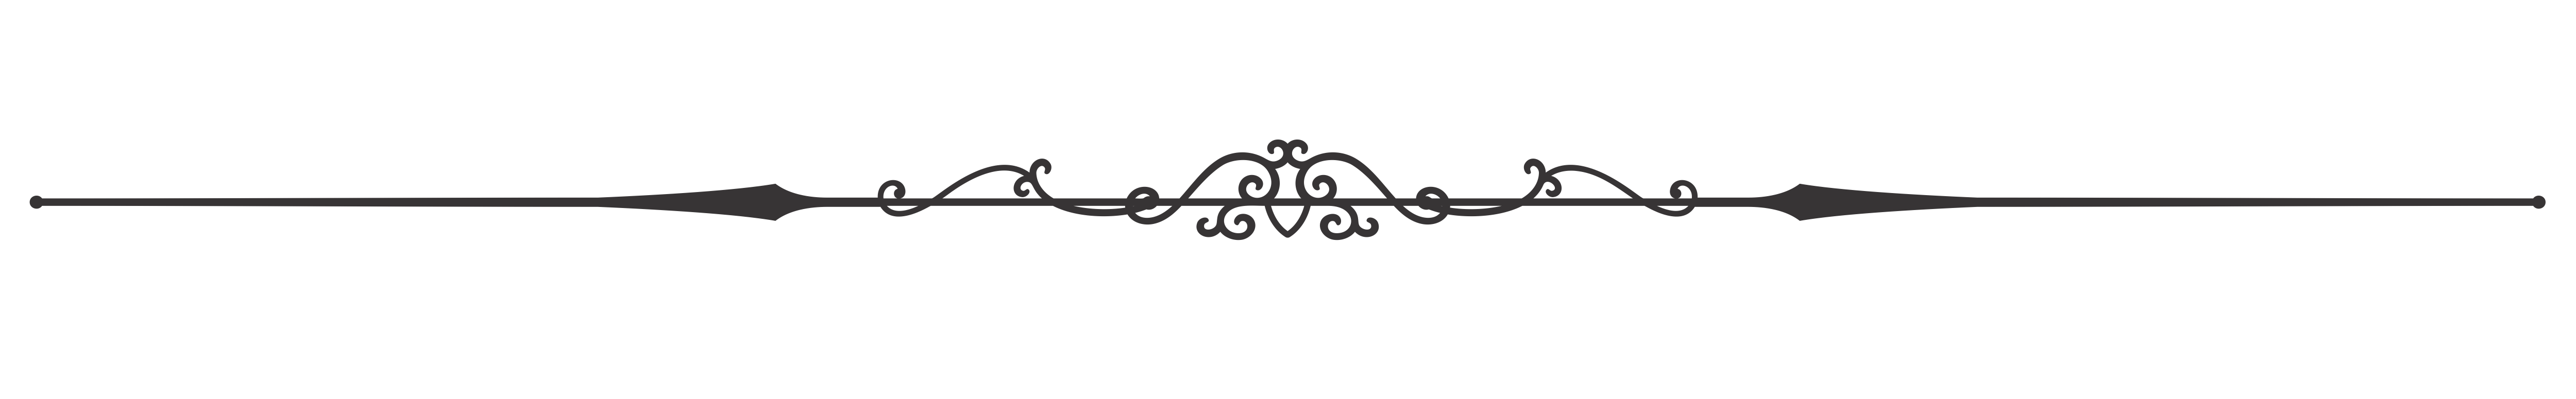
\includegraphics[width=0.75\textwidth]{Screenshots/line.png}
\end{center}
\end{document}